\documentclass[a4paper]{ctexart}
\usepackage{xeCJK}
\usepackage{times}
\usepackage{setspace}
\usepackage{fancyhdr}
\usepackage{graphicx}
\usepackage{wrapfig}
\usepackage{array}
\usepackage{fontspec,xunicode,xltxtra}
\usepackage{titlesec}
\usepackage{titletoc}
\usepackage[titletoc]{appendix}
\usepackage[top=29mm,bottom=29mm,left=30mm,right=30mm]{geometry}
\usepackage{enumerate}
\usepackage{caption}
\usepackage{amsmath,bm}
\usepackage{cite}
\usepackage{enumitem}
\setmainfont{Times New Roman}
\setCJKmainfont[BoldFont={Songti SC Bold}]{SimSun}
\setCJKfamilyfont{heiti}{SimHei}
\renewcommand{\heiti}{\CJKfamily{heiti}\fontspec{Times New Roman}}

\ctexset {
	section = {
		number = \arabic{section},
		format = \zihao{4}\bfseries,
	},
	subsection = {
		number = \arabic{section}.\arabic{subsection},
		format = \zihao{-4}\bfseries,
	}
}


\setlength\parskip{.5\baselineskip}
\fancypagestyle{plain}{\pagestyle{fancy}}%改变章节首页页眉
\pagestyle{fancy}
\lhead{\kaishu~《中外哲学概论与评析》课程作业~}
\rhead{\kaishu~至善1706~尹达恒}
\cfoot{}

\begin{document}
\begin{center}
	{\zihao{-3}\textbf{科技传承者的人生价值}}

	{\zihao{-4}尹达恒}\\[-1mm]

	{\zihao{5}(江南大学物联网工程学院)}
\end{center}
\begin{spacing}{1.3}
	\zihao{-4}
	身为计算机专业的学生,我所学的知识就是和如何机器打交道,我每天面对的东西不是实验室中的瓶瓶罐罐,不是未知的自然谜题,而是一代代人类天才的智慧结晶,是完全非自然的、人类的造物。每当我对自己所学的专业知识产生疑问,想要刨根问底时,能够得到的结果永远只能止步于“前人所创”,而不会被引导到宏大复杂的自然哲学体系中。身在计算机专业,我对自己的身份定位是“承前启后”,学习前人创造的知识,发明新的知识留给后人。因此对我来说,思考人生的意义离不开对传承的思考。

	技术发展和科学探索有所不同,前者更注重于个人的想法与灵感,而后者更偏重于对事实的观察和总结,但它们都有一个共同的特点——传承。不管是技术发明还是科学规律,都能通过某种方式在一代代人类之间传承,下一代人学习了上一代的技术发明和科学规律,在这些知识的基础上又会产生新的技术发明和科学规律,并连同上一代的技术发明和科学规律一道再传承给下一代,人类的技术和科学因此在一代又一代人之间传递与发展。从这个角度上看,每个人虽然都无法逃脱重复的生死循环,但是在整体上,人类的科技却一直在向前发展。既然从人生老病死的生命循环之中难以发掘意义,那么不妨从一直前进的科技发展中探寻人生的意义。
	首先一个最重要的问题是:为什么人会发展科技?这个问题很复杂,因为在现代,科技发展的推动力涉及到人类社会的各方各面,人类的经济政治文化都和科技发展有千丝万缕的联系。但如果对这个问题追根溯源,可以追溯到一个原始问题:为什么人会发明工具?这个问题的答案显而易见:为了更好地生存。在我们的祖先所生活的热带森林中,工具并非生存的必要条件,但即便如此,为了更高效地获取食物,为了更加美好的生活,我们的祖先发明了工具。这个答案在现代科学上同意适用。数千年来,从石器时代到青铜时代,从铁器时代到蒸汽时代,科技发展的最终极目的未曾改变——让人类过上更美好的生活。

	\begin{figure}
		\centering
		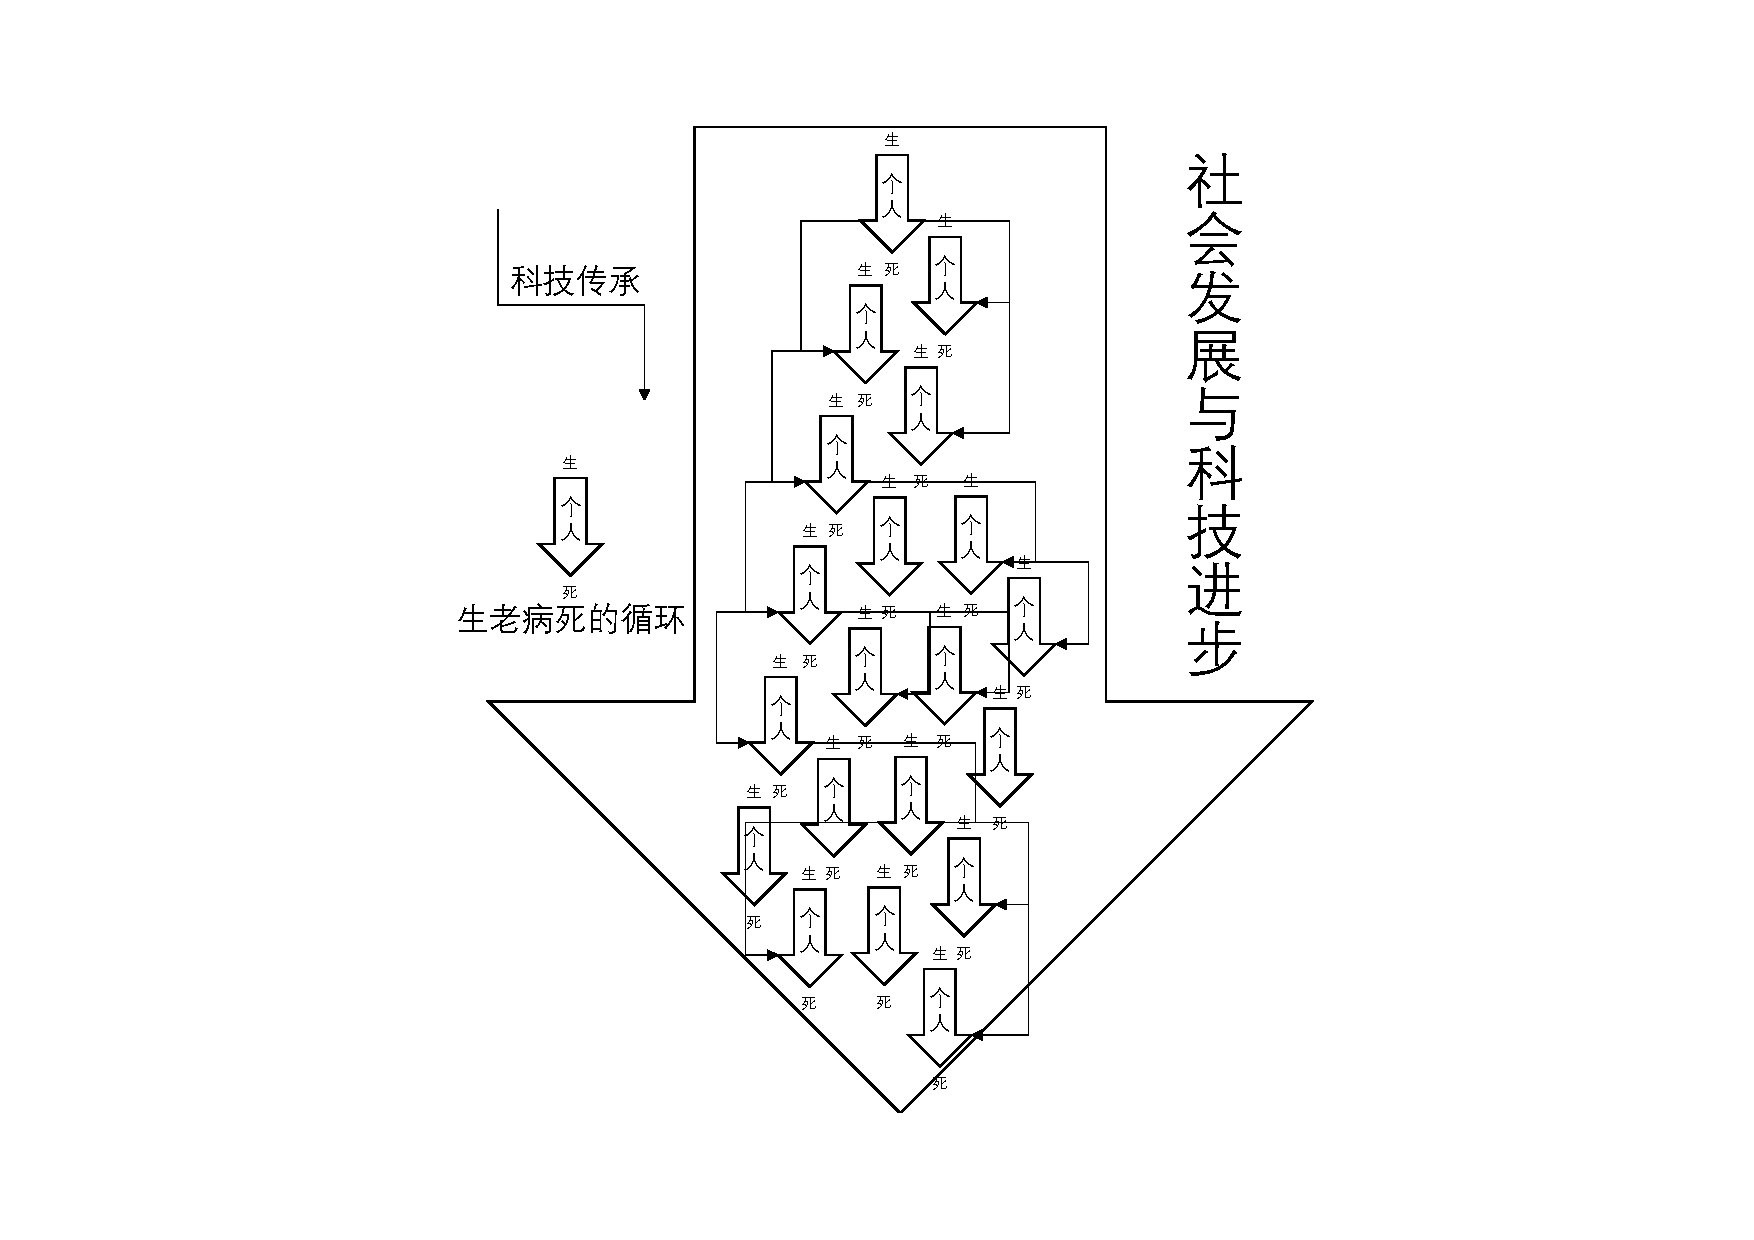
\includegraphics[width=\textwidth, keepaspectratio]{figure/1.pdf}\\
		\caption{生老病死、科技传承与社会进步}
	\end{figure}
	而在科技的发展与传承的过程中,起到决定性作用的就是一代又一代为科技事业穷尽一生的传承者——科学家和工程师们。从这个角度看来,作为一名科技传承者的人生意义也就显而易见了——让人类的生活更加美好,让人类积累的科技继续发展与传承。这是一种既有外在标准又有内在标准的人生意义。“让人类积累的科技继续发展与传承”显然是一个外在的标准,它表示下一代人能记得从前一代人传承下来的知识和上一代人中新出现的知识。而“让人类的生活更加美好”的标准则多种多样,因为科技发展并不是百利而无一害的,许多能造福人类的科技也能被用于战争,而即使是被用于战争的科技也不全会人类带来灾难。因此,科技传承者是否传承了“让人类的生活更加美好”的科技没有一个固定的衡量标准,更多的依赖科学家和工程师自己对科学应用的积累与主观见解。

	人固然无法逃脱生老病死的重复与循环,在一代代人类生老病死的重复与循环中所产生的科技传承确是超越了重复而不断前进的。为了人类更加美好的生活而推动科技的不断进步,便是科技传承者们的人生意义。
\end{spacing}
\end{document}